\chapter{Análise e Desenho da Solução}
\label{sec:3-Analise}

Depois de contextualizados os temas relevantes, o presente capítulo foca-se na análise do problema 
que sustenta este relatório e na apresentação do desenho da solução criada.

\section{Domínio do Problema}

O fluxo que trata da informação de catálogo é dos mais sensíveis e cruciais para o bom funcionamento
dos sistemas que integram os serviços do grupo Flutter. Este fluxo funciona em tempo-real recorrendo
ao uso de \textit{streams} para conseguir atingir este objetivo. Esta abordagem permite garantir
o processamento assíncrono dos dados relativos a este fluxo de uma forma otimizada.

De momento, os serviços responsáveis pelo processamento destes dados estão distribuídos em dois
\textit{\glspl{cluster}} que usam \textit{Apache Storm} para a gestão do mesmo. Esta solução apresenta alguns
defeitos que são importantes de resolver por forma a melhorar a capacidade de escalabilidade destes
serviços. 

O primeiro destes problemas é o elevado número de \acp{VM} presente em cada \textit{\gls{cluster}},
este problema impacta a solução na fase de lançamento de novas versões. Isto deve-se ao facto de
toda a infraestrutura estar sob demanda constante com vários lançamentos paralelos de vários serviços
em ao ser necessário criar novas \acp{VM} o processo responsável pela gestão de máquinas da
infraestrutura pode não ser capaz de responder ao pedido. Desta forma, diminuir o número de \acp{VM}
presentes no \textit{\gls{cluster}} representaria uma melhoria na probabilidade da taxa de sucesso de
lançamento de uma nova versão (em todos os ambientes).

Além disso, o sistema está a usar um excesso de recursos para determinados serviços. Desta forma,
se for possível alterar o \textit{\gls{flavour}} destes \textit{\glspl{cluster}} vai ser possível economizar
recursos. Para atingir este objetivo existem várias abordagens possíveis, como por exemplo, a
alteração do número de \acp{VM} presentes em cada \textit{\gls{cluster}}, a alteração do \textit{\gls{flavour}}
de cada \textit{\gls{cluster}} ou a alteração da distrubuição de serviços por \textit{\gls{cluster}}.

Por fim, vai ser efetuada a atualização da versão de \textit{Apache Storm} de forma a tirar partido
das funcionalidades mais recentes da ferramenta. Assim como nas alterações anteriores, será também
crucial fazer uma análise cuidada da forma como esta atualização vai ser levada a cabo, isto porque
é importante garantir a disponibilidade de todos os serviços durante estas intervenções. 

\todo[inline,color=blue!20]{? Faz sentido falar sobre a aquisiçaõ da nova marca again?}

\section{Engenharia de Requisitos}

A Engenharia de Requisitos é uma área muito relevante no desenvolvimento de \textit{software}, pois 
sustenta a análise dos projetos. Este passo representa o processo de obtenção de requisitos através 
de uma análise do problema e pressupõe a definição das necessidades do cliente na procura de uma 
solução clara que valide a proposta apresentada. Seguindo um processo estruturado e adotando as 
melhores práticas, promovemos uma melhor comunicação entre as várias partes interessadas.

Considerando os aspetos mencionados, nesta secção serão apresentados todos os 
requisitos do sistema identificados e requisitados no início do projeto de maneira a garantir a 
qualidade da solução desenvolvida. Estes requisitos podem ser categorizados em funcionais - 
funcionalidades distintas e essenciais que o sistema deve realizar, e não funcionais - 
restrições impostas para que o sistema realize os requisitos funcionais corretamente.

\subsection{Requisitos Não Funcionais}

Os requisitos não funcionais não se concentram no que o sistema faz, mas sim em como é esperado que
ele funcione. Estes requisitos são essenciais para a qualidade geral, desempenho e usabilidade do 
\textit{software} e têm em conta fatores como o desempenho, a segurança, a confiabilidade e a 
usabilidade.

Os requisitos não funcionais apresentados em seguida, guiam-se pelo modelo FURPS+, um padrão de 
classificação qualitativa das características de um \textit{software} (\textbf{F}unctionality, 
\textbf{U}sability, \textbf{R}eliability, \textbf{P}erformance, \textbf{S}upportability), para uma 
melhor experiência do utilizador. O "\textbf{+}" refere-se a métodos de classificação diferentes, 
como por exemplo, restrições de design, implementação, interface ou físicos.

\vspace{5mm}

\textbf{Funcionalidade}
\begin{itemize}
  \item Encontram-se especificados na subsecção \nameref{sec:3-rf}.
\end{itemize}

\textbf{Usabilidade}
\begin{itemize}
  \item xxx
    \todo[inline]{Perguntar na Blip se há algum requisito enquadrado}
\end{itemize}

\textbf{Confiabilidade}
\begin{itemize}
  \item A aplicação deve ser capaz de recuperar de falhas sem perda de dados.
  \item A aplicação deve ser capaz de recuperar de falhas minimizando o tempo de inatividade.
  \item A aplicação deve ser capaz de recuperar de falhas sem intervenção manual.
\end{itemize}

\textbf{Desempenho}
\begin{itemize}
  \item O sistema deve ser capaz de processar transações em dia de pico sem falhas.
  \item O sistema deve ser capaz de processar transações em dia de pico minimizando o tempo de resposta.
\end{itemize}

\textbf{Suporte}
\begin{itemize}
  \item xxx
    \todo[inline]{Perguntar na Blip se há algum requisito enquadrado}
\end{itemize}

\textbf{Restrições de Design}
\begin{itemize}
  \item O sistema deve suportar quatro ambientes - \ac{QA}, desenvolvimento, 
    performance e produção.
  \item O sistema deve estar replicado em dois \glspl{dc}.
  \item Todas as \acp{VM} do mesmo \textit{\gls{cluster}} devem ter o mesmo \textit{\gls{flavour}}.
  \item A paralelização deve ser feita por \ac{VM} e não por processo. Ou seja, a mesma \ac{VM} 
    não pode ter dois processos a correr em paralelo.
\end{itemize}

\subsection{Requisitos Funcionais}
\label{sec:3-rf}

Os requisitos funcionais especificam as unidades funcionais de um sistema de \textit{software}.
Estes requisitos concentram-se nas funções que devem ser disponibilizadas, descrevem as
funcionalidades, comportamentos e operações específicas que os utilizadores devem ser capazes de 
executar, podendo variar desde ações básicas, como entrada e saída de dados, a algorítmos 
específicos e processos de negócio.

De forma a facilitar a compreensão dos requisitos funcionais estes encontram-se descritos na 
Tabela \ref{tab:reqfun} e na Figura \ref{dcu}, na forma de \textit{User Stories}, seguindo a 
estrutura apresentada no artigo "(User) Stories for Analytics Projects - Part 1". \cite{us}.

\begin{table}[H]
  \begin{center}
    \caption{Requisitos Funcionais}
    \vspace{5mm}
    \label{tab:reqfun}
    \begin{tabular}{|c|l|}
      \hline
      ID & User Story                                                                  \\ \hline
      1  & \begin{tabular}[c]{@{}l@{}}Como Engenheiro de Aplicações, pretendo que seja efetuado \\
        um estudo que determine possíveis otimizações de recursos nos \textit{\glspl{cluster}} dos serviços \\
      de catálogo .\end{tabular} \\ \hline
      2  & \begin{tabular}[c]{@{}l@{}}Como Engenheiro de Aplicações, pretendo que seja elaborado \\
        um plano que defina como serão efetuadas as alterações nos recursos dos \textit{\glspl{cluster}} \\
        dos serviços de catálogo .\end{tabular} \\ \hline
      3  & \begin{tabular}[c]{@{}l@{}}Como Engenheiro de Aplicações, pretendo que sejam efetuadas \\
      reduções de recursos nos \textit{\glspl{cluster}} dos serviços de catálogo atuais.\end{tabular} \\ \hline
      4  & \begin{tabular}[c]{@{}l@{}}Como Engenheiro de Aplicações, pretendo que a versão de \\
        \textit{Apache Storm} utilizada pelos \textit{\glspl{cluster}} dos serviços de catálogo seja atualizada \\
        para a versão mais recente.\end{tabular} \\ \hline
      5  & \begin{tabular}[c]{@{}l@{}}Como XXX, quero XXX.\end{tabular} \\ \hline
    \end{tabular}
  \end{center}
\end{table}

\begin{figure}[H]
  \centerline{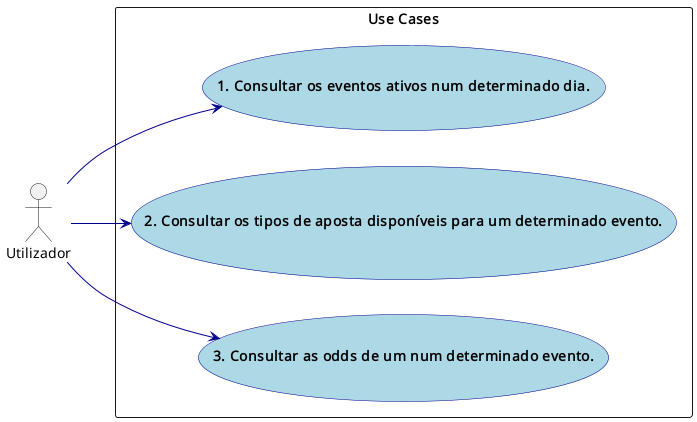
\includegraphics[scale=0.4]{media/content/analise/ucd.png}}
  \caption{Diagrama de Casos de Uso}
  \label{dcu}
\end{figure}

\section{Desenho da Solução}

Após a análise do problema definido juntamente com os requisitos funcionais e não funcionais,
apresentados anteriormente, o objetivo desta secção é documentar as fases que fazem parte do
desenho da solução idealizada.

\todo[inline]{TODO}

